\documentclass{article}
\usepackage{graphicx}
\usepackage[colorlinks]{hyperref}

\title{TC Centers API Documentation}
\date{2018-06-11}
\author{Adrien Pyke}

\begin{document}
	\pagenumbering{gobble}
	\maketitle
	\newpage
	\pagenumbering{arabic}

	\section{Setup}
	\begin{enumerate}
		\item Install \href{https://nodejs.org/en/}{node.js}. The project requires version 8.0 or later.
		\item Open a command prompt, and navigate to the \texttt{tcapi} folder. (\texttt{cd /path/to/folder/tcapi})
		\item Run the command \texttt{npm install} to install the dependencies.
		\item Run the command \texttt{npm start} to start the server.
		\item Access the api at \url{http://localhost:8080/tcapi/centers}.
	\end{enumerate}

	\section{Tips}

	\subsection{Run on a different port}
	By default the server runs on port 8080, but if you'd like to change that, you can open \texttt{.env} and change the value of \texttt{PORT}.

	\subsection{Reset the Database}
	If you'd ever like to reset the database to it's initial state, open a command prompt and run \texttt{node seed.js}.

	\newpage

	\section{Documentation}
	\begin{figure}[h!]
		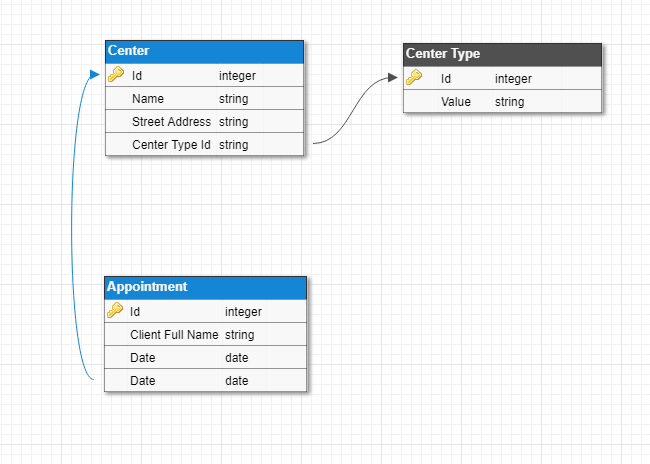
\includegraphics[width=\linewidth]{data-model.png}
		\caption{Conceptual Data Model}
		\label{fig:datamodel}
	\end{figure}
\end{document}
